\section{方法}
\label{chapter:02}

% block-id: 02.conventions.heading
\hypertarget{02.conventions.heading}{}
\subsection{工况与比较量}

% block-id: 02.conventions.p1
\hypertarget{02.conventions.p1}{}
计算采用 SI 单位、exp(jωt) 时间约定和 RMS 相量。材料为 20 ℃ 铜，电导率 σ=5.8×10⁷ S/m，相对磁导率 μr=1；主输运工况为 200 kHz、20 A RMS，独立外加场为零。股线沿途绝缘、端部并联。电阻和损耗按轴向长度归一化，股线的实际弧长另行计入铜体积与直流电阻。有限段端电压的单位为 V，二维轴向端场的单位为 V/m，二者通过所采用的轴向长度建立联系。

% block-id: 02.conventions.p2
\hypertarget{02.conventions.p2}{}
原题 Q1 的直径 2 mm 圆线用于解析校准。其铜面积为 3.141593 mm²，在 20 A 下的平均直流电流密度为 6.366198 A/mm²，超过题设 4 A/mm² 限值。满足该限值的 Q2 需至少 5 mm² 铜截面。640 股、单股铜径 0.100 mm 的理想圆面积为 5.026548 mm²，二维模型以 64 边形表示每股，实际铜面积为 \metric{coax_area} mm²。等铜比较使用实际离散面积，使几何近似的影响与电磁结果具有一致的参照。

% block-id: 02.conventions.p3
\hypertarget{02.conventions.p3}{}
各股具有不同弧长时，直流电阻由并联电导求得，铜体积由各股面积与弧长乘积相加，见 \eqref{eq:E01}。本文同时考察绝对交流电阻、Rac/Rdc、铜损耗与复电流分配。RMS 相量下的焦耳损耗见 \eqref{eq:E02}；该式中电阻由纯输运工况的铜损耗定义。补充材料的 RT0 算例采用独立外场和零净输运，其吸收功率以外场损耗单独报告。

% block-id: 02.equation.E01
\hypertarget{02.equation.E01}{}
\hypertarget{E01}{}
\begin{equation}
\begin{gathered}
R_{\mathrm{dc}}=\left(\sum_{k=1}^{N}\frac{\sigma A_k}{\ell_k}\right)^{-1} \\
V_{\mathrm{Cu}}=\sum_{k=1}^{N}A_k\ell_k
\end{gathered}
\tag{1}\label{eq:E01}
\end{equation}

% block-id: 02.equation.E02
\hypertarget{02.equation.E02}{}
\hypertarget{E02}{}
\begin{equation}
\begin{gathered}
P_{\mathrm{Cu}}=\int_{\Omega_{\mathrm{Cu}}}|\mathbf J|^2/\sigma\,\mathrm d\Omega \\
R_{\mathrm{ac}}=P_{\mathrm{Cu}}/|I_t|^2 \\
r_{\mathrm{ac}}=R_{\mathrm{ac}}/L_z
\end{gathered}
\tag{2}\label{eq:E02}
\end{equation}

% block-id: 02.hierarchy.heading
\hypertarget{02.hierarchy.heading}{}
\subsection{模型层级与验证关系}

% block-id: 02.hierarchy.p1
\hypertarget{02.hierarchy.p1}{}
各模型的关系如 图~\ref{fig:model_hierarchy} 所示。解析圆线与二维扩散模型具有共同的长直内场问题，可比较径向电流和内部电阻。二维共端模型进一步保留股内分布、股间电流与受控回流，适合研究指定截面的场路耦合。纵向 PEEC 采用有限长度部分电感核，可检查长度对轴向电流解的影响。三分量 RT0 模型则以长方体外场吸收为算例，检验三维电流连续性与离散算子。换位路径和实际端区需要相应的沿程或横向自由度，属于后续三维结构研究的范围。

% block-id: 02.figure.model_hierarchy
\hypertarget{02.figure.model_hierarchy}{}
\begin{figure}[!htbp]
\centering
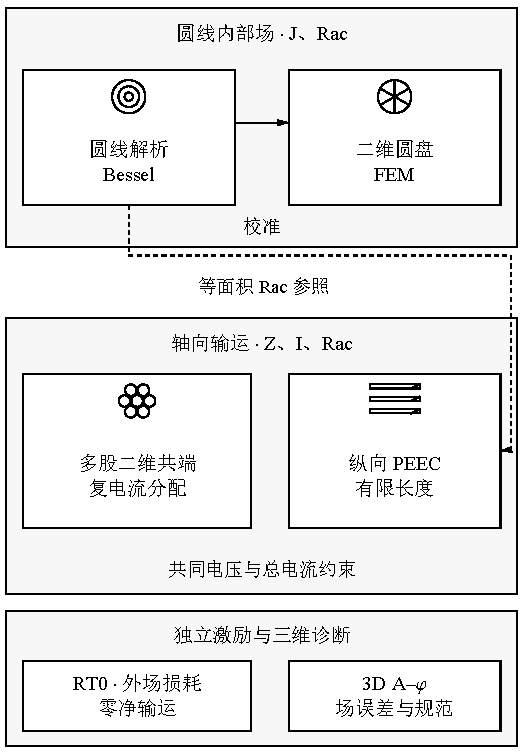
\includegraphics[width=\linewidth,height=.72\textheight,keepaspectratio]{../../assets/zh-CN/model_hierarchy.pdf}
\caption{分层模型与可比较观测量。 输运模型按物理对象与观测量分组：圆线内场用于解析与二维校准，多股二维场路求解共同端口下的复电流，纵向 PEEC 检验有限长度效应。连线标明内部场校准或等面积电阻参照。RT0 外场损耗与三维 A–φ 场诊断各自构成独立研究范围。}
\label{fig:model_hierarchy}
\end{figure}

% block-id: 02.hierarchy.p2
\hypertarget{02.hierarchy.p2}{}
验证分为方程求解、物理约束、功率一致性和参数敏感性四部分。真实线性残差、共同端条件与总复电流误差的目标为 10⁻⁸，独立功率平衡为 0.1\%，网格、分段、边界及长度变化的比较目标为 1\%。解析参考与电流、功率积分分别使用 10⁻⁶ 和 10⁻⁸ 门槛。RT0 的 GMRES 真残差目标为 10⁻¹¹，积分敏感性为 0.1\%；同模型 CPU/GPU 矩阵与复电流的对照门槛为 10⁻¹⁰。

% block-id: 02.hierarchy.p3
\hypertarget{02.hierarchy.p3}{}
这些检查回答不同的问题。残差衡量离散系统的求解精度，功率平衡检查场路与后处理的一致性，参数敏感性表征指定扰动范围内的变化。模型遗漏、边界近似及实验偏差需要相应的独立证据。因此，下文分别说明数值检查结果及其物理适用范围，并把有限敏感性结果作为局部验证，而非全模型误差的统一上界。

% block-id: 02.common.heading
\hypertarget{02.common.heading}{}
\subsection{共端场路与复电流均流条件}

% block-id: 02.common.p1
\hypertarget{02.common.p1}{}
共同端点、股线支路与回流的关系见 图~\ref{fig:common_terminal}。令 Z 为指定线性模型的耦合阻抗矩阵，e 为独立外场引起的感应项，i 为各股复电流，V 为公共端电压。端口方程 Z i+e=V1 与总电流条件 1\(^{\mathrm T}\)i=It 共同构成 \eqref{eq:E04}。求解该增广系统可同时得到幅值和相位，等流值 It/N 用于比较求得的电流分布。

% block-id: 02.equation.E04
\hypertarget{02.equation.E04}{}
\hypertarget{E04}{}\begin{equation}\begin{bmatrix} Z&-\mathbf1\\ \mathbf1^T&0\end{bmatrix}\begin{bmatrix}\mathbf i\\V\end{bmatrix}=\begin{bmatrix}-\mathbf e\\I_t\end{bmatrix}\tag{3}\label{eq:E04}\end{equation}

% block-id: 02.figure.common_terminal
\hypertarget{02.figure.common_terminal}{}
\begin{figure}[!htbp]
\centering
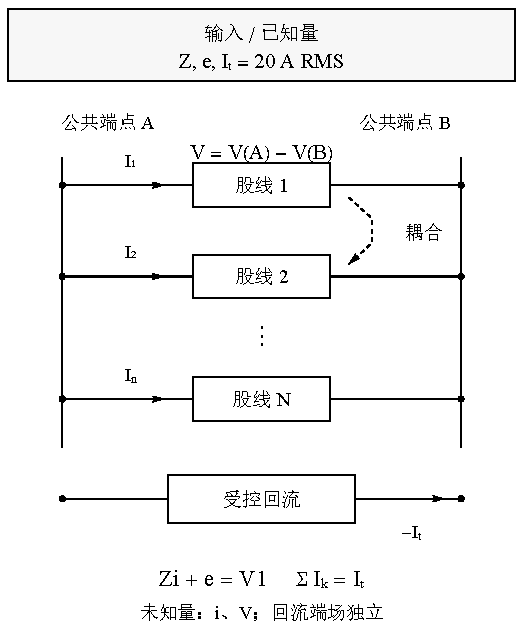
\includegraphics[width=\linewidth,height=.72\textheight,keepaspectratio]{../../assets/zh-CN/common_terminal.pdf}
\caption{多股共同端口与回流。 各股沿途绝缘，在两端并联，逐股复电流由共同端电压及总电流约束求解。耦合矩阵 Z 与激励项 e 包含指定模型中的阻抗和场作用。受控回流承担反向总电流，并具有独立的端场。图中给出已知输入及待求复电流和电压。}
\label{fig:common_terminal}
\end{figure}

% block-id: 02.common.p2
\hypertarget{02.common.p2}{}
在增广系统具有唯一解时，令 i=(It/N)1 可知：等流解存在，当且仅当向量 (It/N)Z1+e 的所有分量相同。将该向量投影到与 1 正交的子空间，便得到 \eqref{eq:E05}。无独立外场时，条件简化为 Z 的各行和相同；存在外场时，感应项也参与决定均流。该判据给出了所选阻抗模型与端接条件下的充要条件，便于将几何换位的作用具体落实到耦合矩阵及感应项的变化上。

% block-id: 02.equation.E05
\hypertarget{02.equation.E05}{}
\hypertarget{E05}{}
\begin{equation}
\begin{gathered}
Q=I_N-\mathbf1\mathbf1^T/N \\
Q\left[(I_t/N)Z\mathbf1+\mathbf e\right]=\mathbf0
\end{gathered}
\tag{4}\label{eq:E05}
\end{equation}

% block-id: 02.common.p3
\hypertarget{02.common.p3}{}
二维共端 FEM 将公共轴向端场与 Az 自由度联合求解。导体内按 Jz=σ(v−u) 恢复电流密度，其中 v 与保存变量 u 均以 V/m 表示，回流导体使用相应的端场。电流和损耗由带材料标记的线性三角形积分，坐标由 mm 转换为 m 后计算面积。由此得到的逐股复电流、束内损耗、回流损耗及铜面积，与原始场路结果独立核对；空气区域与各导体区域分别处理。

% block-id: 02.peec_method.heading
\hypertarget{02.peec_method.heading}{}
\subsection{有限长度纵向 PEEC}

% block-id: 02.peec_method.p1
\hypertarget{02.peec_method.p1}{}
纵向 PEEC 将导体截面离散为体积细丝，每条细丝内采用沿轴向、沿长度均匀的复电流密度。欧姆电阻与有限体积对的部分电感由 \eqref{eq:E08} 给出，并形成 Z=R+jωL，随后按 \eqref{eq:E04} 施加公共端口和总电流约束。1264 与 5024 表示体积细丝自由度；这些细丝是连续导体的离散单元。同一截面内各体积细丝的电流差异表示内部电流集中，所用基函数的范围为纵向电流。

% block-id: 02.equation.E08
\hypertarget{02.equation.E08}{}
\hypertarget{E08}{}
\begin{equation}
\begin{gathered}
R_{\alpha\beta}=\delta_{\alpha\beta}\frac{L_z}{\sigma A_\alpha} \\
L_{\alpha\beta}=\frac{\mu}{4\pi A_\alpha A_\beta}\int_{V_\alpha}\int_{V_\beta}\frac{\hat{\mathbf t}_\alpha\cdot\hat{\mathbf t}_\beta}{|\mathbf r-\mathbf r'|}\,\mathrm dV\,\mathrm dV'
\end{gathered}
\tag{5}\label{eq:E08}
\end{equation}

% block-id: 02.peec_method.p2
\hypertarget{02.peec_method.p2}{}
纵向算例的名义圆线直径为 2 mm。m40 与 m80 的方形细丝宽度分别为 0.050 mm 和 0.025 mm，对应实际截面面积 3.16 mm² 和 3.14 mm²。敏感性试验分别改变长度、互项积分或自项积分设置。1264 自由度模型采用同一截面与 0.16、0.32、0.64 m 三档长度；固定长度后，将互项积分阶数 q 依次取为 4、6、8，自项精度从 10/8 提高至 12/10；两个数字依次表示自项数值积分的 AccuracyGoal 与 PrecisionGoal，即绝对精度和相对精度的目标位数。5024 自由度模型复核 0.32、0.64 m 长度及相同积分变化。两种截面离散的铜面积略有差异，因此各档电阻分别与自身等面积圆线的 Bessel 解比较；跨档变化同时包含离散和面积近似的影响。

% block-id: 02.peec_method.p3
\hypertarget{02.peec_method.p3}{}
部分电感核包含有限导体周围的磁耦合，圆线 Bessel 解给出长直导体的内部阻抗。两者在本文中以耗散分量 Rac 进行比较，同时保留长度和面积条件。长度试验衡量当前核与纵向基函数的敏感性；横向环流、曲线股线和真实端部电流重分布需通过扩展自由度研究。与 FEM–PEEC 耦合方法 \cite{P03} 的联系在于场路联合描述，具体的激励、回流和场反馈方式仍应按各实现分别比较。
